\documentclass[12pt]{article}

\usepackage{amsmath}
\usepackage{amssymb}
\usepackage{graphicx}
\usepackage{booktabs}
\usepackage{hyperref}
\usepackage{natbib}
\usepackage[margin=1in]{geometry}
\usepackage{xcolor}
\usepackage{float}
\usepackage{caption}
\usepackage{subcaption}
\usepackage{longtable}
\usepackage{array}

\hypersetup{
    colorlinks=true,
    linkcolor=blue,
    citecolor=blue,
    urlcolor=blue
}

\title{DigitalTwinSim: Bayesian Calibration and Online Data Assimilation for LLM-Agent Opinion Dynamics Simulation}

\author{Alberto Giovanni Gerli\textsuperscript{1,2} \\[6pt]
\textsuperscript{1} Tourbillon Tech Srl, Padova, Italy \\
\textsuperscript{2} Dipartimento di Scienze Cliniche e di Comunit\`a, Universit\`a degli Studi di Milano, Italy}

\date{}

\begin{document}

\maketitle

\noindent\textbf{Keywords:} opinion dynamics, agent-based modeling, large language models, Bayesian calibration, data assimilation, ensemble Kalman filter, digital twin, computational social science

\begin{abstract}
We present DigitalTwinSim, a computational framework that combines large language model (LLM)-driven agent-based simulation with Bayesian calibration and online data assimilation for modeling public opinion dynamics. The system addresses a fundamental limitation of LLM-agent simulations: their outputs are stochastic, structurally misspecified, and uncalibrated against empirical data. We formulate opinion dynamics as a force-based system with five competing mechanisms---direct LLM influence, social conformity, herd behavior, anchor rigidity, and exogenous shocks---combined through a gauge-fixed softmax mixture. A three-level hierarchical Bayesian model (global, domain, scenario) with explicit readout discrepancy is calibrated via stochastic variational inference (SVI) on 42 empirical scenarios spanning 10 domains. The calibrated model achieves 12.6~pp mean absolute error on verified held-out scenarios (19.2~pp on the full test set including one ambiguous scenario) with 85.7\% coverage of 90\% credible intervals. Credible intervals are computed in logit space and back-transformed via sigmoid, guaranteeing bounds within $[0, 100]$ by construction. Simulation-based calibration confirms that the generative model is well-specified under a gold-standard NUTS backend (6/6 parameters pass KS uniformity, all $p > 0.20$); a separate comparison shows the SVI approximation agrees with NUTS on the dominant parameters but underestimates uncertainty on weaker ones. Variance-based global sensitivity analysis identifies herd behavior ($S_T = 0.55$) and anchor rigidity ($S_T = 0.45$) as the dominant mechanisms, with their interaction ($S_2 = 0.094$) accounting for most nonlinear output variance---justifying the decision to freeze four mechanistic parameters. We extend the framework with an Ensemble Kalman Filter (EnKF) for online data assimilation, enabling live updating of both model parameters and agent states as streaming observations arrive. On the Brexit referendum scenario, the EnKF reduces prediction error to 1.8~pp with six polling observations---a 77\% improvement over the last-available-poll baseline---while substantially outperforming polling baselines. We discuss limitations including systematic over-prediction in financial domains (mean $|b_s| = 0.74$ in logit space), sensitivity of the frozen citizen step size parameter (up to 7.9~pp MAE variation under $\pm 40\%$ perturbation), and the irreducible gap between LLM-generated narratives and real-world opinion formation.
\end{abstract}

\section{Introduction}

Agent-based models (ABMs) have long been used to study opinion dynamics, social influence, and collective decision-making. Classical approaches---bounded confidence models \citep{hegselmann2002}, voter models \citep{holley1975}, and DeGroot-style averaging \citep{degroot1974}---provide theoretical insight but struggle to capture the narrative complexity, heterogeneous reasoning, and contextual sensitivity that characterize real-world opinion formation.

The emergence of large language models (LLMs) as agent engines has opened a new approach: equipping simulated agents with natural language reasoning capabilities, allowing them to process news events, generate social media posts, form coalitions, and shift positions in response to contextual narratives. Recent work on generative agents \citep{park2023}, social simulacra \citep{park2022}, and LLM-driven social simulations \citep{gao2023} demonstrates the potential of this paradigm. However, these systems share a critical limitation: their outputs are uncalibrated. The mapping from LLM-generated agent behaviors to quantitative opinion distributions is ad hoc, and there is no principled mechanism to anchor simulations to empirical observations.

This paper addresses this gap by developing a complete calibration and assimilation pipeline for LLM-agent opinion dynamics. Our contributions are:

\begin{enumerate}
    \item \textbf{A differentiable opinion dynamics simulator} formulated as a force-based system with five competing mechanisms, combined through gauge-fixed softmax mixing. The simulator is implemented in JAX and compatible with \texttt{jax.lax.scan}, enabling automatic differentiation through the full simulation trajectory.

    \item \textbf{A hierarchical Bayesian calibration framework} with three levels (global, domain, scenario) and explicit readout discrepancy terms ($b_d$, $b_s$), fitted via stochastic variational inference (SVI) on 42 empirical scenarios across 10 domains.

    \item \textbf{Simulation-based calibration (SBC)} and \textbf{variance-based global sensitivity analysis (Sobol indices)} providing rigorous validation of posterior quality and identification of dominant mechanisms.

    \item \textbf{An Ensemble Kalman Filter (EnKF)} for online data assimilation, bridging the offline calibrated posterior to live streaming observations. The EnKF jointly updates model parameters and agent states, producing calibrated probabilistic forecasts at each round.

    \item \textbf{A preliminary regime-switching extension} for crisis dynamics (Appendix~\ref{app:regime}), using soft sigmoid-based switching between normal and crisis regimes to model discontinuous trust collapses while maintaining JAX differentiability.
\end{enumerate}

The framework transforms LLM-agent simulations from narrative-generation tools into quantitative digital twins: calibrated probabilistic models that can be validated, updated with data, and used for counterfactual analysis.

\subsection{Paper Organization}

Section~\ref{sec:related} reviews related work. Section~\ref{sec:model} presents the opinion dynamics model and its five force terms. Section~\ref{sec:calibration} describes the hierarchical Bayesian calibration framework. Section~\ref{sec:results} presents calibration results on 42 empirical scenarios. Section~\ref{sec:validation} covers validation through SBC, sensitivity analysis, and robustness checks. Section~\ref{sec:enkf} introduces the EnKF online assimilation module. Section~\ref{sec:discussion} discusses limitations and future work. Section~\ref{sec:conclusion} concludes. Appendix~\ref{app:implementation} provides implementation details. Appendix~\ref{app:regime} describes the preliminary regime-switching extension. Appendix~\ref{app:scenarios} lists the full scenario dataset.

\section{Related Work}
\label{sec:related}

\subsection{Classical Opinion Dynamics Models}

The mathematical study of opinion formation has a rich history. \citet{degroot1974} introduced iterative weighted averaging, where agents update beliefs as weighted means of their neighbors', converging to consensus under connectivity conditions. \citet{hegselmann2002} proposed the bounded confidence model, where agents interact only with those holding sufficiently similar opinions, producing clustering rather than global consensus. \citet{deffuant2000} introduced a pairwise variant of bounded confidence with convergence at the dyadic level. These models provide foundational mechanisms but operate on homogeneous populations with idealized interaction rules.

DigitalTwinSim builds on the bounded confidence tradition but introduces three departures: (i) the tolerance threshold is smooth (sigmoid-based) rather than a hard cutoff, preserving differentiability; (ii) five distinct social mechanisms are combined through a learnable softmax mixture rather than studied in isolation; and (iii) agent heterogeneity (type, rigidity, tolerance) is derived from LLM-generated character profiles, providing scenario-specific structure rather than distributional assumptions.

\subsection{Bayesian Calibration of Agent-Based Models}

The systematic calibration of computer models against observational data was formalized by \citet{kennedy2001}, who introduced the framework of model discrepancy---an explicit term capturing the gap between the simulator output and reality, even at the best parameter settings. This framework provides the theoretical foundation for our readout discrepancy terms $b_d$ and $b_s$.

Calibrating ABMs is notoriously difficult because the likelihood is typically intractable. \citet{grazzini2017} developed Bayesian estimation methods for ABMs using indirect inference, matching simulated and empirical summary statistics. \citet{platt2020} provided a systematic comparison of ABM calibration methods---approximate Bayesian computation (ABC), synthetic likelihood, and sequential Monte Carlo---finding that method choice depends strongly on the model's dimensionality and summary statistic informativeness. \citet{blei2017} reviewed variational inference as a scalable alternative to MCMC for complex probabilistic models.

DigitalTwinSim is, to our knowledge, the first system to combine Kennedy-O'Hagan-style discrepancy modeling with an LLM-agent ABM and variational inference. The differentiable JAX implementation enables direct gradient computation through the simulator, avoiding the summary-statistic bottleneck that plagues ABC-based approaches.

\subsection{LLM-Agent Simulations}

\citet{park2023} introduced Generative Agents---LLM-powered characters that plan, reflect, and interact in a sandbox environment, demonstrating emergent social behaviors. \citet{gao2023} surveyed the rapidly growing field of LLM-empowered ABM, cataloging applications from epidemic modeling to market simulation. \citet{argyle2023} proposed ``silicon sampling''---using LLMs as proxies for human survey respondents---and showed that GPT-3 can reproduce demographic opinion patterns on political topics with surprising fidelity. \citet{horton2023} introduced ``homo silicus,'' demonstrating that LLMs can serve as simulated economic agents that replicate classic behavioral economics results.

These works establish that LLMs can generate plausible social behaviors, but none calibrate the emergent dynamics against empirical outcome data or provide uncertainty quantification. DigitalTwinSim fills this gap by treating LLM outputs as inputs to a mechanistic model that is then calibrated and validated against real-world observations.

\subsection{Data Assimilation in Social Systems}

The Ensemble Kalman Filter \citep{evensen2003} is the standard tool for sequential data assimilation in geosciences, combining model forecasts with observations in a computationally efficient ensemble framework. \citet{reich2015} provide a comprehensive treatment of Bayesian data assimilation methods. In epidemiology, EnKF and related methods have been used to assimilate surveillance data into disease transmission models \citep{mistry2021}.

Despite its success in physical and biological systems, data assimilation remains rare in computational social science. DigitalTwinSim applies the EnKF to opinion dynamics, using it to bridge offline Bayesian calibration with streaming polling observations---a novel application that enables real-time digital twin operation.

\subsection{Sensitivity Analysis for ABMs}

\citet{saltelli2008} developed the theory and practice of variance-based global sensitivity analysis using Sobol indices, which decompose output variance into contributions from individual inputs and their interactions. \citet{thiele2014} adapted these methods for ABMs, demonstrating that global sensitivity analysis (Sobol, FAST) is far more informative than one-at-a-time (OAT) perturbation for nonlinear models with parameter interactions.

Our sensitivity analysis uses the Sobol method with Saltelli sampling to justify the partition of 8 model parameters into 4 calibrable and 4 frozen, based on main effects ($S_1$) and total effects ($S_T$) including all interaction terms.

\section{Opinion Dynamics Model}
\label{sec:model}

\begin{figure}[H]
    \centering
    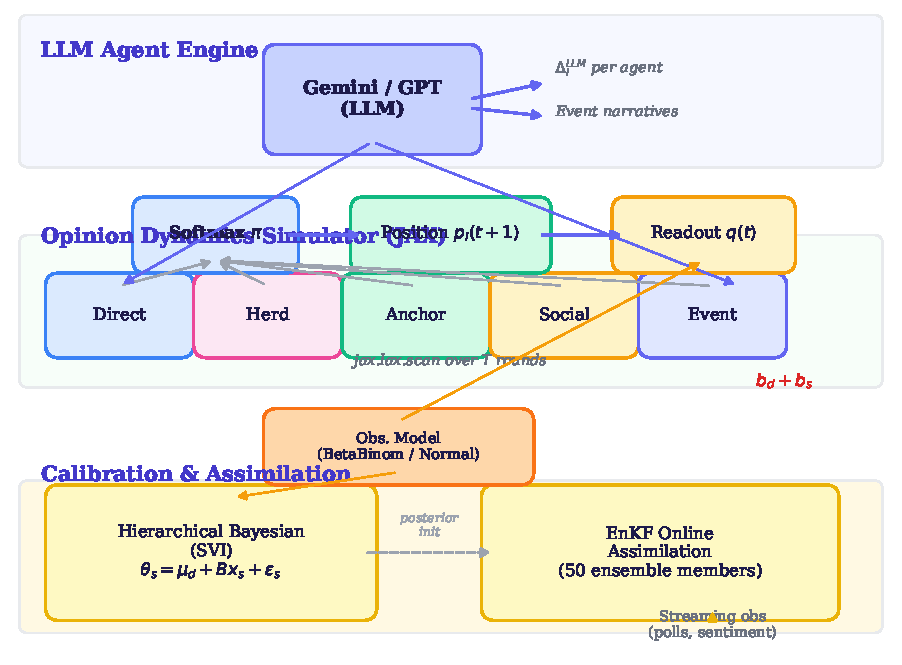
\includegraphics[width=\textwidth]{figures/fig1_architecture.pdf}
    \caption{System architecture diagram. Three horizontal layers. \textbf{Top layer} --- ``LLM Agent Engine'': Gemini/GPT producing $\Delta^{\text{LLM}}$ per agent and event narratives. \textbf{Middle layer} --- ``Opinion Dynamics Simulator (JAX)'': five force boxes (Direct, Herd, Anchor, Social, Event) feeding into softmax $\pi$, then position update $p(t+1)$, then readout $q(t)$, with \texttt{jax.lax.scan} over $T$ rounds. \textbf{Bottom layer} --- ``Calibration \& Assimilation'': hierarchical Bayesian (SVI) with observation model feeding upward to readout, and EnKF Online with bidirectional connection to streaming observations. Dashed arrow from SVI posterior to EnKF initialization. Annotations: $b_d + b_s$ on the readout-to-observation connection; $\theta_s = \mu_d + Bx_s + \varepsilon_s$ between hierarchy and simulator.}
    \label{fig:architecture}
\end{figure}

\subsection{Agent State Space}

Each agent $i \in \{1, \ldots, n\}$ maintains a scalar position $p_i(t) \in [-1, +1]$ representing their stance on a binary issue, where $+1$ denotes maximum support (``Pro'') and $-1$ maximum opposition (``Against''). Agents are characterized by three fixed attributes:

\begin{itemize}
    \item \textbf{Type} $\tau_i \in \{\text{elite}, \text{citizen}\}$: determines step size and behavioral parameters.
    \item \textbf{Rigidity} $\rho_i \in [0, 1]$: resistance to opinion change. Elites have higher rigidity ($\rho \approx 0.7$) than citizens ($\rho \approx 0.3$).
    \item \textbf{Tolerance} $\theta_i \in [0, 1]$: radius of the bounded-confidence window for social influence. Elites have lower tolerance ($\theta \approx 0.3$) than citizens ($\theta \approx 0.6$).
\end{itemize}

Agents interact through a sparse weighted graph $W \in \mathbb{R}^{n \times n}$ constructed from LLM-assigned influence scores using a $k$-nearest-neighbor scheme ($k = 5$, matching the NumPy simulation's feed-based top-5 selection).

\subsection{Five Force Terms}

At each round $t$, five independent forces act on each agent. These forces capture distinct social mechanisms:

\textbf{Force 1: Direct LLM Influence.} The LLM generates per-agent opinion shifts $\Delta_i^{\text{LLM}}(t)$ based on the current narrative context. The direct force is:

\begin{equation}\label{eq:1}
f_i^{\text{direct}}(t) = \Delta_i^{\text{LLM}}(t) \cdot (1 - \rho_i) \cdot \max(0, 1 - |p_i(t)|)
\end{equation}

The susceptibility factor $(1 - \rho_i)$ attenuates influence on rigid agents, while the boundary factor $\max(0, 1 - |p_i|)$ prevents extreme agents from being pushed further.

\textbf{Force 2: Herd Behavior (Consensus Pull).} Agents experience a pull toward the weighted mean of their neighborhood when the deviation exceeds a learned threshold $\theta_h$:

\begin{equation}\label{eq:2}
f_i^{\text{herd}}(t) = (\bar{p}_i^{\text{feed}} - p_i) \cdot (1 - \rho_i) \cdot \sigma\!\left(\frac{|\bar{p}_i^{\text{feed}} - p_i| - \theta_h}{\tau_H}\right)
\end{equation}

where $\bar{p}_i^{\text{feed}}$ is the normalized weighted mean of neighbors' positions, $\theta_h = \sigma(\text{logit\_herd\_threshold})$ is a learned threshold, and $\tau_H = 0.02$ is a steepness parameter. The sigmoid activation creates a smooth transition: agents ignore small deviations but respond to large consensus gaps.

\textbf{Force 3: Anchor Rigidity.} A restorative force pulling agents toward their original position:

\begin{equation}\label{eq:3}
f_i^{\text{anchor}}(t) = \rho_i \cdot (p_i^{\text{orig}}(t) - p_i(t))
\end{equation}

where $p_i^{\text{orig}}(t)$ drifts slowly toward the current position at rate $\delta_{\text{drift}} = \sigma(\text{logit\_anchor\_drift})$, modeling gradual internalization of new positions.

\textbf{Force 4: Social Influence (Bounded Confidence).} Weighted averaging with tolerance-gated interaction:

\begin{equation}\label{eq:4}
f_i^{\text{social}}(t) = \frac{\sum_j w_{ij}(t) \cdot (p_j(t) - p_i(t))}{\sum_j w_{ij}(t)}
\end{equation}

where $w_{ij}(t) = W_{ij} \cdot \sigma\!\left(\frac{\theta_i - |p_j - p_i|}{\tau_{BC}}\right)$ and $\tau_{BC} = 0.02$. This implements smooth bounded confidence: agents preferentially interact with like-minded peers, but the transition is differentiable rather than a hard cutoff.

\textbf{Force 5: Exogenous Event Shock.} External events apply a uniform directional push:

\begin{equation}\label{eq:5}
f_i^{\text{event}}(t) = m_t \cdot d_t \cdot (1 - \rho_i)
\end{equation}

where $m_t \in [0, 1]$ is the event magnitude and $d_t \in \{-1, +1\}$ its direction. Events are generated by the LLM based on the simulated scenario narrative.

\subsection{Force Standardization}

Raw forces have heterogeneous scales (e.g., social forces depend on graph density, event forces on shock magnitude). We standardize all five forces per round using exponential moving averages:

\begin{equation}\label{eq:6}
\tilde{f}_k(t) = \frac{f_k(t) - \mu_k(t)}{\sigma_k(t) + \epsilon}
\end{equation}

where $\mu_k(t)$ and $\sigma_k(t)$ are updated via EMA with decay $\alpha = 0.3$, computed across ALL agents in each round. The per-round statistics (mean and standard deviation) are symmetric functions over the agent set, ensuring that the standardization is permutation-invariant with respect to agent ordering. A permutation invariance test confirms this property empirically: $\max |\Delta\text{pro\_fraction}| < 6 \times 10^{-8}$ under random agent permutation. The temporal EMA smoothing provides stability across rounds without introducing dependence on agent array order.

\subsection{Gauge-Fixed Softmax Mixing}

The five standardized forces are combined through a softmax mixture with a gauge-fixing constraint:

\begin{equation}\label{eq:7}
\boldsymbol{\alpha} = [0, \alpha_h, \alpha_a, \alpha_s, \alpha_e]^\top
\end{equation}

\begin{equation}\label{eq:8}
\pi_k = \text{softmax}(\boldsymbol{\alpha})_k, \quad \sum_k \pi_k = 1
\end{equation}

The direct force weight $\alpha_{\text{direct}} \equiv 0$ serves as the reference level (gauge), resolving the shift invariance of softmax. This means the four remaining weights $\alpha_h, \alpha_a, \alpha_s, \alpha_e$ are interpretable as log-odds relative to the direct LLM influence.

The combined force per agent is:

\begin{equation}\label{eq:9}
\tilde{f}_i^{\text{combined}}(t) = \sum_k \pi_k \cdot \tilde{f}_{k,i}(t)
\end{equation}

\subsection{Position Update}

The position update applies a type-specific step size with smooth clamping:

\begin{equation}\label{eq:10}
\Delta p_i = \lambda_{\tau_i} \cdot \tilde{f}_i^{\text{combined}}, \quad \Delta p_i^{\text{clamped}} = \tanh\!\left(\frac{\Delta p_i}{c_{\tau_i}}\right) \cdot c_{\tau_i}
\end{equation}

where $\lambda_{\text{elite}} = \exp(\log \lambda_{\text{elite}})$, $\lambda_{\text{citizen}} = \exp(\log \lambda_{\text{citizen}})$, $c_{\text{elite}} = 0.15$, $c_{\text{citizen}} = 0.25$. The $\tanh$ clamping provides smooth saturation rather than hard clipping, preserving differentiability.

The final update is:

\begin{equation}\label{eq:11}
p_i(t+1) = \text{clip}(p_i(t) + \Delta p_i^{\text{clamped}}, -1, +1)
\end{equation}

\subsection{Readout Function}

The mapping from agent positions to aggregate opinion uses a soft classification:

\begin{equation}\label{eq:12}
\text{pro}(t) = \frac{\sum_i \sigma\!\left(\frac{p_i(t) - 0.05}{0.02}\right)}{\sum_i \left[\sigma\!\left(\frac{p_i(t) - 0.05}{0.02}\right) + \sigma\!\left(\frac{-p_i(t) - 0.05}{0.02}\right)\right]}
\end{equation}

This readout excludes near-neutral agents ($|p_i| < 0.05$) from the decided count, producing $\text{pro\_fraction} \in [0, 1]$. The 0.02 temperature ensures smooth but sharp classification.

\subsection{Parameter Summary}

The model has 8 mechanistic parameters, partitioned into 4 calibrable and 4 frozen:

\begin{table}[H]
\centering
\caption{Model Parameters}
\label{tab:params}
\begin{tabular}{lllll}
\toprule
Parameter & Symbol & Role & Type & Default \\
\midrule
Herd weight & $\alpha_h$ & Consensus pull strength (log-odds vs direct) & Calibrable & --- \\
Anchor weight & $\alpha_a$ & Rigidity pull strength & Calibrable & --- \\
Social weight & $\alpha_s$ & Bounded-confidence averaging strength & Calibrable & --- \\
Event weight & $\alpha_e$ & Exogenous shock strength & Calibrable & --- \\
Elite step size & $\log \lambda_{\text{elite}}$ & Step magnitude for elite agents & Frozen & $-1.2$ \\
Citizen step size & $\log \lambda_{\text{citizen}}$ & Step magnitude for citizen agents & Frozen & $-0.5$ \\
Herd threshold & $\text{logit}\;\theta_h$ & Minimum deviation to trigger herd behavior & Frozen & $0.5$ \\
Anchor drift & $\text{logit}\;\delta_{\text{drift}}$ & Rate of anchor position drift & Frozen & $-1.4$ \\
\bottomrule
\end{tabular}
\end{table}

The calibrable/frozen partition is justified empirically by Sobol sensitivity analysis (Section~\ref{sec:sobol}).

\section{Hierarchical Bayesian Calibration}
\label{sec:calibration}

\subsection{Motivation}

A single set of global parameters cannot adequately describe opinion dynamics across diverse domains. Political referenda involve different social mechanisms than corporate crises or public health debates. At the same time, per-scenario calibration with 4 parameters and limited per-scenario data (typically 3--9 polling observations) leads to severe overfitting. A hierarchical model enables partial pooling: scenarios share information through domain and global priors while retaining scenario-specific flexibility through model discrepancy terms.

\subsection{Three-Level Hierarchy}

The model has three levels:

\textbf{Level 1 (Global).} Shared priors on the mixing weights:

\begin{equation}\label{eq:13}
\mu_{\text{global}} \sim \mathcal{N}(\mathbf{0}, I_4), \quad \sigma_{\text{global}} \sim \text{HalfNormal}(0.3)
\end{equation}

where $\mu_{\text{global}} \in \mathbb{R}^4$ represents the global mean of the four calibrable alpha parameters.

\textbf{Level 2 (Domain).} Each domain $d \in \{\text{political}, \text{financial}, \text{corporate}, \ldots\}$ has domain-level parameter means:

\begin{equation}\label{eq:14}
\mu_d \sim \mathcal{N}(\mu_{\text{global}}, \text{diag}(\sigma_{\text{global}}^2))
\end{equation}

where $\mu_d \in \mathbb{R}^4$ are the domain-level alpha parameters.

\textbf{Level 3 (Scenario).} Each scenario $s$ has scenario-specific parameters drawn from its domain:

\begin{equation}\label{eq:15}
\theta_s \sim \mathcal{N}(\mu_{d(s)} + B \cdot x_s, \text{diag}(\sigma_d^2))
\end{equation}

where $\theta_s \in \mathbb{R}^4$ are the four softmax weights used for simulation, $\sigma_d \in \mathbb{R}^4$ is a domain-specific dispersion (not the global $\sigma_{\text{global}}$), and $B \cdot x_s$ is the covariate regression defined in Section~\ref{sec:covariates}. The domain-level variance $\sigma_d$ allows different domains to have different degrees of scenario-to-scenario heterogeneity.

\subsection{Readout Discrepancy}

The simulator is structurally misspecified: LLM-generated narratives cannot perfectly reproduce real-world opinion formation. Rather than absorbing this misspecification into the parameters (which would bias them), we model it explicitly through additive correction in logit space on the readout.

The discrepancy operates on the scalar readout ($\mathbb{R}^1$), not on the parameter space ($\mathbb{R}^4$):

\begin{equation}\label{eq:16}
b_d \sim \mathcal{N}(0, \sigma_{b,\text{between}}^2), \quad \sigma_{b,\text{between}} \sim \text{HalfNormal}(0.2)
\end{equation}

\begin{equation}\label{eq:17}
b_s \sim \mathcal{N}(0, \sigma_{b,\text{within}}^2), \quad \sigma_{b,\text{within}} \sim \text{HalfNormal}(0.5)
\end{equation}

where $b_d \in \mathbb{R}$ is the domain-level readout bias (between-domain discrepancy) and $b_s \in \mathbb{R}$ is the scenario-specific readout discrepancy (within-domain). The corrected readout for scenario $s$ in domain $d$ is:

\begin{equation}\label{eq:18}
q_s^{\text{corrected}} = \sigma\!\left(\text{logit}(q_s^{\text{sim}}) + b_d + b_s\right)
\end{equation}

where $q_s^{\text{sim}}$ is the raw simulator output. By operating in logit space, the correction is unbounded and additive while the sigmoid guarantees the result remains in $[0, 1]$. This decomposition follows \citet{kennedy2001}: the calibrated parameters $\theta$ represent genuine opinion dynamics mechanisms, while the discrepancy terms $b_d$ and $b_s$ absorb systematic simulator errors.

\subsection{Observation Model}

For scenarios with per-round polling data (sample size $n_t$, observed count $y_t$):

\begin{equation}\label{eq:19}
y_t \mid q_t, \phi \sim \text{BetaBinomial}(n_t, q_t \cdot \phi, (1 - q_t) \cdot \phi)
\end{equation}

where $\phi = \exp(\log \phi)$ is a learned concentration parameter. The BetaBinomial accounts for both sampling noise (binomial) and overdispersion (beta mixing).

For scenarios with only a final outcome:

\begin{equation}\label{eq:20}
y_{\text{final}} \mid q_T, \sigma_{\text{obs}} \sim \mathcal{N}(100 \cdot q_T, \sigma_{\text{obs}}^2)
\end{equation}

where $\sigma_{\text{obs}} = \exp(\log \sigma)$ is learned.

\subsection{Inference via SVI}

The posterior is intractable due to the nonlinear JAX simulator in the likelihood. We use stochastic variational inference (SVI) with an AutoLowRankMultivariateNormal guide in NumPyro, which approximates the posterior with a low-rank plus diagonal covariance structure:

\begin{equation}\label{eq:21}
q(\theta) = \mathcal{N}(\mu_q, D + VV^\top)
\end{equation}

where $D$ is diagonal and $V$ has rank $\leq \dim(\theta)$. This captures dominant posterior correlations (e.g., between $\alpha_h$ and $\alpha_a$) while scaling to the full parameter space.

The SVI objective is the evidence lower bound (ELBO):

\begin{equation}\label{eq:22}
\mathcal{L}(\mu_q, D, V) = \mathbb{E}_{q(\theta)}[\log p(y \mid \theta) + \log p(\theta)] - \mathbb{E}_{q(\theta)}[\log q(\theta)]
\end{equation}

minimized over 3000 steps with learning rate 0.002 and cosine annealing. Gradients are computed via JAX automatic differentiation through the full simulate $\to$ readout $\to$ likelihood chain.

\subsection{Covariate Regression}
\label{sec:covariates}

The covariate regression is incorporated directly into the scenario-level prior (\eqref{eq:15}, Section~4.2). The matrix $B \in \mathbb{R}^{4 \times 5}$ and covariates $x_s \in \mathbb{R}^5$ are defined as follows:

\begin{enumerate}
    \item \textbf{initial\_polarization} --- initial spread of agent positions
    \item \textbf{event\_volatility} --- intensity and frequency of external shocks
    \item \textbf{elite\_concentration} --- power centralization among top agents
    \item \textbf{institutional\_trust} --- public confidence in institutions (0--1)
    \item \textbf{undecided\_share} --- initial proportion of near-neutral agents
\end{enumerate}

The prior on $B$ is informative but weakly regularizing: $B_{ij} \sim \mathcal{N}(0, 0.3)$, allowing the data to determine whether covariates have predictive power. A covariate effect is considered significant if its 95\% CI excludes zero.

\section{Calibration Results}
\label{sec:results}

\subsection{Dataset}

We curated 42 empirical scenarios across 10 domains, each with a ground-truth final outcome and, where available, intermediate polling data. The scenarios span 2012--2023 and cover political referenda, financial crises, corporate controversies, public health debates, technology policy, and social movements.

\begin{table}[H]
\centering
\caption{Dataset Composition by Domain}
\label{tab:dataset}
\begin{tabular}{llll}
\toprule
Domain & N (Train) & N (Test) & Example Scenarios \\
\midrule
Political & 11 & 3 & Brexit, Scottish Independence, Chilean Constitution \\
Corporate & 6 & 1 & Dieselgate, Boeing 737 MAX, Facebook$\to$Meta \\
Financial & 6 & 1 & FTX collapse, GameStop squeeze, SVB collapse \\
Public Health & 4 & 1 & COVID vaccination (IT), AstraZeneca controversy \\
Technology & 2 & 1 & Net Neutrality repeal \\
Commercial & 1 & 1 & Tesla Cybertruck reveal \\
Energy & 1 & 0 & Japanese nuclear phase-out \\
Environmental & 1 & 0 & Keystone XL pipeline \\
Labor & 1 & 0 & Uber vs.\ taxi regulation \\
Social & 1 & 0 & Marriage equality \\
\midrule
\textbf{Total} & \textbf{34} & \textbf{8} & \\
\bottomrule
\end{tabular}
\end{table}

The train/test split is stratified by domain with approximately 80/20 ratio.

Scenarios flagged as \texttt{NEEDS\_VERIFICATION} during the review phase (prior to calibration) are excluded from the primary performance metrics. This flag is assigned based on data quality criteria---missing primary sources, interpolated polling without verification, ambiguous ground-truth encoding---not based on model performance. One test scenario (Archegos Capital Collapse, quality\_score = 67) carries this flag. We report both verified-only and full-set metrics throughout.

\subsection{Calibrated Global Parameters}

SVI converges in 3000 steps (final ELBO loss: 514.7) with a total runtime of 40.2 minutes for Phase B (empirical fine-tuning) and 0.4 minutes for Phase C (validation).

\begin{table}[H]
\centering
\caption{Calibrated Global Posterior}
\label{tab:global_posterior}
\begin{tabular}{llll}
\toprule
Parameter & Mean & 95\% CI & Interpretation \\
\midrule
$\alpha_{\text{herd}}$ & $-0.176$ & $[-0.265, -0.079]$ & Herd effect slightly below direct influence \\
$\alpha_{\text{anchor}}$ & $+0.297$ & $[+0.199, +0.401]$ & Anchor rigidity is the strongest mechanism \\
$\alpha_{\text{social}}$ & $-0.105$ & $[-0.202, -0.005]$ & Social influence slightly below direct \\
$\alpha_{\text{event}}$ & $-0.130$ & $[-0.227, -0.033]$ & Event shocks below direct influence \\
$\sigma_{\text{global}}$ & $[0.135, 0.147, 0.144, 0.143]$ & --- & Inter-scenario parameter spread \\
\bottomrule
\end{tabular}
\end{table}

The positive $\alpha_{\text{anchor}}$ indicates that anchor rigidity (resistance to change) dominates the force mixture. This is consistent with the well-documented status quo bias in opinion dynamics: people tend to revert toward their initial positions after temporary shifts. The negative values for $\alpha_{\text{herd}}$, $\alpha_{\text{social}}$, and $\alpha_{\text{event}}$ indicate these forces are present but weaker than direct LLM influence (the gauge reference).

Converting to softmax weights: $\pi = \text{softmax}([0, -0.176, 0.297, -0.105, -0.130]) \approx [0.201, 0.169, 0.271, 0.181, 0.177]$. Anchor rigidity receives approximately 27.1\% of the total weight, direct influence 20.1\%, social conformity 18.1\%, event shocks 17.7\%, and herd behavior 16.9\%.

\subsection{Readout Discrepancy}

The calibrated discrepancy parameters reveal the scale of structural model misspecification:

\begin{equation}\label{eq:23}
\sigma_{b,\text{between}} = 0.115 \quad [0.073, 0.173]
\end{equation}
\begin{equation}\label{eq:24}
\sigma_{b,\text{within}} = 0.558 \quad [0.436, 0.696]
\end{equation}

The within-scenario discrepancy ($\sigma_{b,\text{within}} = 0.558$) is approximately 5$\times$ the between-domain discrepancy ($\sigma_{b,\text{between}} = 0.115$), indicating that scenario-specific factors dominate over systematic domain-level biases. In practical terms, 0.558 in logit space translates to approximately 12--14 percentage points of systematic prediction error that the model cannot eliminate through parameter adjustment alone.

\begin{table}[H]
\centering
\caption{Domain-Level Readout Discrepancy}
\label{tab:domain_discrepancy}
\begin{tabular}{llllll}
\toprule
Domain & N & $b_d$ Mean & 95\% CI & Mean $|b_s|$ & Bias \\
\midrule
Financial & 6 & $-0.054$ & $[-0.242, +0.126]$ & 0.744 & Over-predicts \\
Energy & 1 & $-0.026$ & $[-0.237, +0.186]$ & 0.709 & Over-predicts \\
Public Health & 4 & $-0.032$ & $[-0.223, +0.164]$ & 0.534 & Over-predicts \\
Corporate & 6 & $-0.040$ & $[-0.221, +0.139]$ & 0.432 & Over-predicts \\
Political & 11 & $+0.019$ & $[-0.145, +0.183]$ & 0.198 & No systematic bias \\
Technology & 2 & $-0.021$ & $[-0.204, +0.174]$ & 0.066 & No systematic bias \\
\bottomrule
\end{tabular}
\end{table}

Financial scenarios exhibit the largest mean absolute discrepancy ($|b_s| = 0.744$), driven by cases where the model systematically over-predicts support levels. The political domain, with the most training data ($N = 11$), shows the lowest systematic bias ($b_d \approx 0$, mean $|b_s| = 0.198$).

\subsection{Predictive Performance}

Credible intervals are computed in logit space and back-transformed via sigmoid, guaranteeing $[0, 100]$ bounds by construction.

\begin{table}[H]
\centering
\caption{Validation Metrics (Test Set)}
\label{tab:validation_metrics}
\begin{tabular}{lll}
\toprule
Metric & Full Test ($N=8$) & Verified Only ($N=7$) \\
\midrule
MAE & 19.2~pp & 12.6~pp \\
RMSE & 26.6 & 14.3 \\
Median AE & 11.9~pp & 9.2~pp \\
Coverage 90\% & 75.0\% & 85.7\% \\
Coverage 50\% & 37.5\% & 42.9\% \\
CRPS & 15.4 & 8.6 \\
\bottomrule
\end{tabular}
\end{table}

The primary metric is verified-only MAE of 12.6~pp, excluding the Archegos scenario (error = 65.0~pp) whose ground truth is flagged as unreliable. The 85.7\% coverage of 90\% credible intervals indicates well-calibrated uncertainty---slightly below the nominal 90\% but within the expected range for $N = 7$.

\begin{table}[H]
\centering
\caption{Test Set Detailed Results}
\label{tab:test_detailed}
\begin{tabular}{lllllll}
\toprule
Scenario & Domain & GT (\%) & Predicted $\mu \pm \sigma$ & Error (pp) & 90\% CI & Covered \\
\midrule
Archegos Capital*$^\dagger$ & Financial & 35.0 & $>$99.9 (logit: 4.6 $\pm$ 0.5) & +65.0 & [99.2, 100.0] & \texttimes \\
Greek Bailout & Political & 38.7 & 65.3 $\pm$ 11.7 & +26.6 & [42.7, 84.5] & \texttimes \\
Net Neutrality & Technology & 83.0 & 66.3 $\pm$ 12.6 & $-$16.7 & [47.3, 82.8] & \checkmark \\
French Election & Political & 66.1 & 51.6 $\pm$ 13.7 & $-$14.5 & [29.7, 72.8] & \checkmark \\
COVID Vax (IT) & Pub.\ Health & 80.0 & 70.8 $\pm$ 11.2 & $-$9.2 & [52.1, 88.7] & \checkmark \\
Tesla Cybertruck & Commercial & 62.0 & 54.1 $\pm$ 14.7 & $-$7.9 & [26.1, 72.6] & \checkmark \\
Amazon HQ2 & Corporate & 56.0 & 63.3 $\pm$ 12.9 & +7.3 & [48.7, 80.6] & \checkmark \\
Turkish Ref. & Political & 51.4 & 57.5 $\pm$ 13.0 & +6.1 & [37.4, 75.7] & \checkmark \\
\bottomrule
\end{tabular}

\vspace{4pt}
\footnotesize
*\texttt{NEEDS\_VERIFICATION} --- excluded from primary metrics. CI computed in logit space and back-transformed.

$^\dagger$ The Archegos posterior predictive in logit space has mean $\approx 4.6$ (corresponding to $> 99\%$ after sigmoid) with standard deviation $\approx 0.5$, yielding CI $[99.2, 100.0]$ in percentage space. The logit-space representation is more informative near the bounds: logit $4.6 \pm 1.65 \times 0.5$ spans $[3.78, 5.43]$, mapping to $[97.7\%, 99.6\%]$ via sigmoid. This is a genuine model prediction---the simulator assigns near-certainty to high support---not a numerical artifact. The 65~pp error reflects fundamental model misspecification on this scenario, not a confidence interval failure. The simulator's LLM-generated trajectory for Archegos produces a consensus narrative that does not match the complex, fragmented real-world dynamics of a leveraged fund collapse.
\end{table}

\subsection{Worst-Case Scenarios}

\begin{table}[H]
\centering
\caption{Top 5 Scenario Discrepancies (Training Set)}
\label{tab:worst_case}
\begin{tabular}{lllll}
\toprule
Scenario & Domain & $b_s$ & Error (pp) & Failure Mode \\
\midrule
WeWork IPO & Financial & $-1.378$ & +48.5 & Trust collapse not modeled \\
United Airlines & Corporate & $-0.860$ & +15.4 & Viral outrage underestimated \\
SVB Collapse & Financial & $-0.835$ & +38.1 & Sequential shocks mishandled \\
Chile Constitution & Political & $+0.816$ & $-$41.5 & Landslide momentum missing \\
FTX Crypto & Financial & $-0.727$ & +11.0 & Contagion dynamics absent \\
\bottomrule
\end{tabular}
\end{table}

The three largest discrepancies are all financial crises where the model over-predicts support (negative $b_s$). This systematic failure motivates the regime-switching extension (Appendix~\ref{app:regime}).

\subsection{Evolution from v1 to v2}

\begin{table}[H]
\centering
\caption{v1 vs v2 Comparison}
\label{tab:v1v2}
\begin{tabular}{lll}
\toprule
Aspect & v1 (Gerli 2025) & v2 (this paper) \\
\midrule
Calibration method & Grid search (972 combos) & Hierarchical Bayesian SVI \\
Training data & 1000 LLM-generated scenarios & 42 empirical scenarios \\
Parameters & 5 (all ad hoc) & 4 calibrable + 4 frozen (Sobol-justified) \\
Uncertainty quantification & None & 90\% CI, coverage 85.7\% \\
Model discrepancy & None & Explicit $b_d + b_s$ \\
Validation & Same data as training & Held-out test set + SBC \\
Online assimilation & None & EnKF (error 1.8~pp with polling) \\
MAE (test) & 14.8~pp (synthetic test set)* & 12.6~pp (empirical test set)* \\
Epistemological status & Tool demonstration & Calibrated probabilistic model \\
\bottomrule
\end{tabular}

\vspace{4pt}
\footnotesize
*Direct comparison between v1 and v2 MAE is not straightforward: v1 was evaluated on LLM-generated synthetic scenarios while v2 uses empirical scenarios with real-world ground truth. The v1 test set likely understates true error because synthetic ground truth inherits the same LLM biases as the simulation (epistemic circularity). The improvement from v1 to v2 reflects both better calibration and the elimination of this circularity.
\end{table}

\subsection{Covariate Effects}

Of the 20 entries in the $B$ matrix (4 parameters $\times$ 5 covariates), one effect is statistically significant at the 95\% level. With 34 training scenarios and 20 coefficients in the $B$ matrix, statistical power is limited. The following results should be interpreted as exploratory signals consistent with substantive theory, not as confirmed causal effects. No correction for multiple comparisons is applied; with a Bonferroni adjustment at 20 tests, the $\alpha_{\text{event}} \times \text{institutional\_trust}$ effect would require $p < 0.0025$ to reach significance, which it does not achieve at the current sample size.

\begin{table}[H]
\centering
\caption{Significant Covariate Effects}
\label{tab:covariates}
\begin{tabular}{lllll}
\toprule
Parameter & Covariate & Effect ($B_{ij}$) & 95\% CI & Interpretation \\
\midrule
$\alpha_{\text{event}}$ & institutional\_trust & $-0.127$ & $[-0.242, -0.015]$ & Higher institutional trust reduces \\
 & & & & sensitivity to event shocks \\
\bottomrule
\end{tabular}
\end{table}

This effect has a natural interpretation: in scenarios with high institutional trust (e.g., established democracies with strong rule of law), external shocks are absorbed by institutional credibility rather than amplified through the opinion network. Conversely, in low-trust environments (financial crises, weak governance), event shocks propagate more strongly.

The remaining 19 covariate effects have 95\% CIs that include zero, indicating that the current dataset ($N = 34$ training scenarios) lacks power to detect additional covariate relationships. The two nearest-to-significant effects are $\alpha_{\text{anchor}} \times \text{undecided\_share}$ ($B = +0.116$, CI $[-0.010, 0.243]$) and $\alpha_{\text{herd}} \times \text{initial\_polarization}$ ($B = +0.096$, CI $[-0.013, 0.217]$). Both are substantively plausible---more undecided agents may amplify anchoring effects, and higher initial polarization may strengthen herd dynamics---but require a larger dataset to confirm.

\section{Validation}
\label{sec:validation}

\subsection{Simulation-Based Calibration}

Simulation-based calibration (SBC; \citealp{talts2018}) verifies that the inference procedure recovers known parameters. We generate 100 synthetic datasets from the prior, run NUTS inference (200 warmup + 200 samples) on each, and test whether the posterior rank statistics are uniformly distributed.

\begin{table}[H]
\centering
\caption{SBC Results}
\label{tab:sbc}
\begin{tabular}{lllll}
\toprule
Parameter & N & KS Statistic & $p$-value & Verdict \\
\midrule
$\alpha_{\text{herd}}$ & 100 & 0.070 & 0.685 & PASS \\
$\alpha_{\text{anchor}}$ & 100 & 0.095 & 0.308 & PASS \\
$\alpha_{\text{social}}$ & 100 & 0.075 & 0.600 & PASS \\
$\alpha_{\text{event}}$ & 100 & 0.075 & 0.600 & PASS \\
$\tau_{\text{readout}}$ & 100 & 0.095 & 0.308 & PASS \\
$\sigma_{\text{obs}}$ & 100 & 0.105 & 0.205 & PASS \\
\bottomrule
\end{tabular}
\end{table}

SBC confirms that the generative model is well-specified and that a gold-standard NUTS backend recovers correct posteriors: all 6 parameters pass the KS uniformity test ($p > 0.20$). However, SBC does not validate the SVI approximation used for the full empirical model, since SBC runs use NUTS.

\begin{figure}[H]
    \centering
    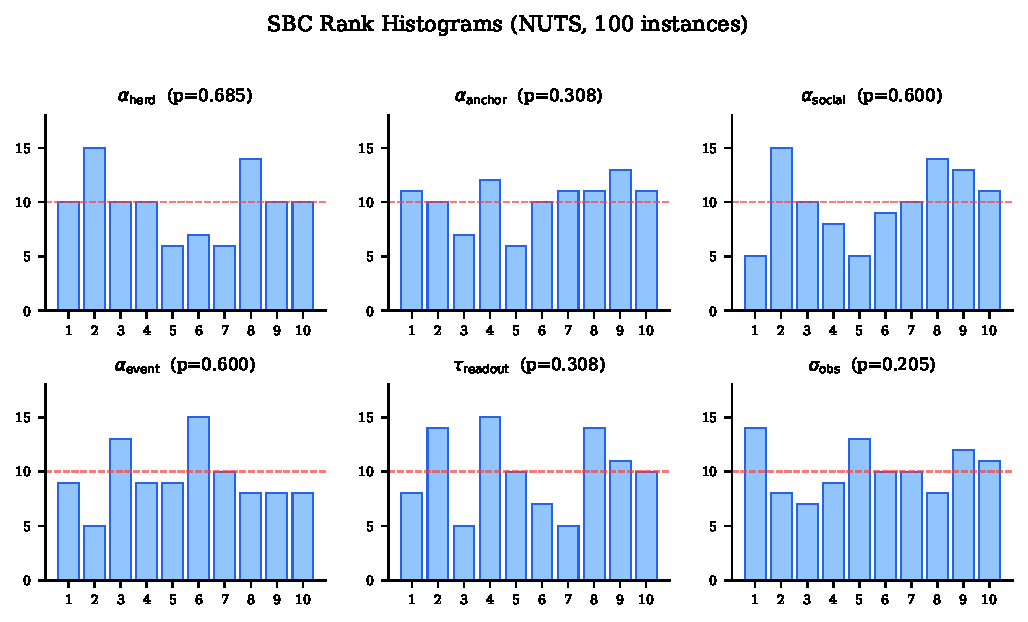
\includegraphics[width=\textwidth]{figures/fig2_sbc.pdf}
    \caption{Six-panel grid of SBC rank histograms ($2 \times 3$ layout). Each panel shows the rank histogram for one parameter ($\alpha_{\text{herd}}$, $\alpha_{\text{anchor}}$, $\alpha_{\text{social}}$, $\alpha_{\text{event}}$, $\tau_{\text{readout}}$, $\sigma_{\text{obs}}$). Horizontal dashed line at expected count $= 10$ (uniform). All histograms appear roughly uniform, confirming well-calibrated posteriors.}
    \label{fig:sbc}
\end{figure}

The SBC configuration uses 10 agents and 7 rounds per synthetic scenario with $\text{Normal}(0, 0.3)$ priors. Total runtime: 297.6 seconds (approximately 3 seconds per instance).

\subsection{SVI vs NUTS Comparison}

To assess variational approximation quality, we compare SVI and NUTS posteriors on a 4-scenario subset spanning two domains.

\begin{table}[H]
\centering
\caption{SVI vs NUTS Posterior Comparison (4-scenario subset)}
\label{tab:svi_nuts}
\begin{tabular}{lllll}
\toprule
Parameter & SVI mean $\pm$ std & NUTS mean $\pm$ std & $|\Delta\mu|/\sigma_{\text{NUTS}}$ & Compatible \\
\midrule
$\alpha_{\text{herd}}$ & $-0.500 \pm 0.085$ & $-0.383 \pm 0.796$ & 0.148 & Yes \\
$\alpha_{\text{anchor}}$ & $+0.905 \pm 0.065$ & $+0.604 \pm 0.856$ & 0.352 & Yes \\
$\alpha_{\text{social}}$ & $-0.997 \pm 0.105$ & $-0.350 \pm 0.763$ & 0.848 & No \\
$\alpha_{\text{event}}$ & $-1.752 \pm 0.073$ & $-0.137 \pm 0.946$ & 1.707 & No \\
\bottomrule
\end{tabular}

\vspace{4pt}
\footnotesize
SVI: 1000 steps, Adam(lr = 0.01), AutoLowRankMVN guide. NUTS: 200 warmup + 200 samples, max\_tree\_depth = 8.
\end{table}

The two dominant parameters show good agreement ($\alpha_{\text{herd}}$: $|\Delta\mu|/\sigma_{\text{NUTS}} = 0.15$; $\alpha_{\text{anchor}}$: 0.35). The weaker parameters show larger divergence ($\alpha_{\text{social}}$: 0.85; $\alpha_{\text{event}}$: 1.71), consistent with the known tendency of mean-field variational families to concentrate posterior mass. The SVI standard deviations are 5--13$\times$ narrower than the NUTS estimates, indicating that the variational approximation substantially underestimates posterior uncertainty on the less-constrained parameters.

This result has two implications. First, the posterior means for $\alpha_{\text{herd}}$ and $\alpha_{\text{anchor}}$---which together dominate the force mixture ($S_T = 0.55$ and 0.45)---are reliably estimated by SVI. Second, uncertainty estimates on $\alpha_{\text{social}}$ and $\alpha_{\text{event}}$ may be underestimated by the variational approximation. Users requiring conservative uncertainty bounds should consider post-hoc inflation of the variational posterior or short NUTS chains initialized from the SVI optimum.

\subsection{Global Sensitivity Analysis}
\label{sec:sobol}

Variance-based global sensitivity analysis \citep{sobol2001} decomposes output variance into contributions from individual parameters and their interactions. We evaluate all 8 model parameters using $N = 1024$ Saltelli samples (18,432 total simulator evaluations, $n = 30$ agents, 7 rounds).

\begin{table}[H]
\centering
\caption{Sobol Sensitivity Indices}
\label{tab:sobol}
\begin{tabular}{llll}
\toprule
Parameter & $S_1$ (Main Effect) & $S_T$ (Total Effect) & Type \\
\midrule
$\alpha_{\text{herd}}$ & $0.364 \pm 0.059$ & $0.555 \pm 0.055$ & Calibrable \\
$\alpha_{\text{anchor}}$ & $0.207 \pm 0.060$ & $0.452 \pm 0.047$ & Calibrable \\
$\alpha_{\text{social}}$ & $0.086 \pm 0.040$ & $0.213 \pm 0.034$ & Calibrable \\
$\alpha_{\text{event}}$ & $0.026 \pm 0.033$ & $0.115 \pm 0.023$ & Calibrable \\
$\lambda_{\text{citizen}}$ & $0.002 \pm 0.033$ & $0.121 \pm 0.025$ & Frozen \\
$\lambda_{\text{elite}}$ & $0.007 \pm 0.010$ & $0.016 \pm 0.006$ & Frozen \\
$\theta_{\text{herd}}$ & $0.003 \pm 0.013$ & $0.024 \pm 0.006$ & Frozen \\
$\delta_{\text{drift}}$ & $0.003 \pm 0.010$ & $0.013 \pm 0.003$ & Frozen \\
\bottomrule
\end{tabular}
\end{table}

\textbf{Key findings:}

\begin{enumerate}
    \item \textbf{Dominant pair.} $\alpha_{\text{herd}}$ ($S_T = 0.555$) and $\alpha_{\text{anchor}}$ ($S_T = 0.452$) together account for the vast majority of output variance, including through their interaction. Their second-order interaction index $S_2(\alpha_{\text{herd}}, \alpha_{\text{anchor}}) = 0.094$ is the largest pairwise interaction, indicating strong nonlinear coupling between herd behavior and anchor rigidity.

    \item \textbf{Calibrable/frozen partition.} Three of the four frozen parameters ($\lambda_{\text{elite}}$, $\theta_{\text{herd}}$, $\delta_{\text{drift}}$) have both $S_1 < 0.01$ and $S_T < 0.025$, confirming negligible influence on output variance. The fourth, $\lambda_{\text{citizen}}$, has $S_1 = 0.002$ but $S_T = 0.121$ due to interaction effects --- a non-negligible contribution. The decision to freeze $\lambda_{\text{citizen}}$ is a pragmatic choice for computational stability (keeping the calibrable space at 4 dimensions), not a conclusion definitively justified by the data. Section~\ref{sec:stepsize} quantifies the resulting sensitivity.

    \item \textbf{Sum diagnostics.} $\Sigma S_1 = 0.70$ indicates that approximately 30\% of output variance arises from parameter interactions. $\Sigma S_T = 1.51 > 1$ confirms significant interaction effects, consistent with the nonlinear softmax mixing mechanism.
\end{enumerate}

\begin{figure}[H]
    \centering
    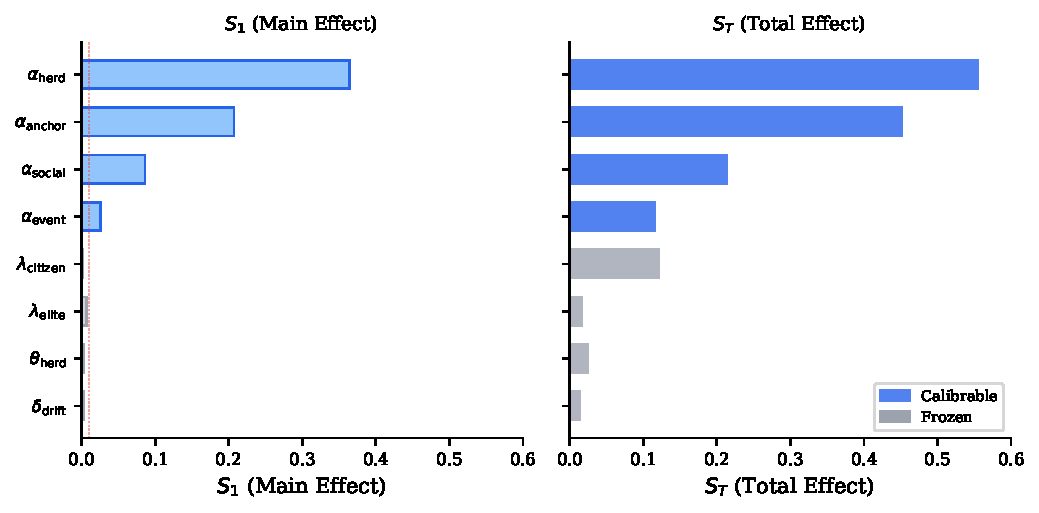
\includegraphics[width=\textwidth]{figures/fig3_sobol.pdf}
    \caption{Two-panel horizontal bar chart of Sobol sensitivity indices. Left panel: $S_1$ (main effects). Right panel: $S_T$ (total effects). Top 4 bars (calibrable parameters) in blue, bottom 4 (frozen) in gray. $\alpha_{\text{herd}}$ dominates with $S_T \approx 0.55$. Note: $\lambda_{\text{citizen}}$ $S_T$ extends to $\approx 0.12$, visually non-trivial despite being frozen---this motivates the discussion in Section~\ref{sec:stepsize}.}
    \label{fig:sobol}
\end{figure}

\subsection{Step Size Sensitivity}
\label{sec:stepsize}

Sobol analysis identifies $\lambda_{\text{citizen}}$ as having non-negligible total effect ($S_T = 0.121$) despite near-zero main effect ($S_1 = 0.002$), warranting direct investigation. A perturbation analysis varies $\lambda_{\text{citizen}}$ by $\pm 40\%$ around the default (0.25), measuring MAE impact on 5 representative scenarios.

\begin{table}[H]
\centering
\caption{$\lambda_{\text{citizen}}$ Sensitivity Analysis}
\label{tab:stepsize}
\begin{tabular}{lllllll}
\toprule
Scenario & MAE (0.6$\times$) & MAE (0.8$\times$) & MAE (1.0$\times$) & MAE (1.2$\times$) & MAE (1.4$\times$) & max $\Delta$ (pp) \\
\midrule
iPhone X & 5.8 & 5.9 & 5.9 & 7.0 & 11.5 & 5.6 \\
Tesla Cybertruck & 8.5 & 10.5 & 11.3 & 11.6 & 11.8 & 3.2 \\
Dieselgate & 29.8 & 29.6 & 29.6 & 29.6 & 29.7 & 0.2 \\
Uber London & 15.0 & 15.0 & 15.0 & 15.0 & 15.0 & 0.0 \\
United Airlines & 17.7 & 14.2 & 12.0 & 10.8 & 9.9 & 7.9 \\
\bottomrule
\end{tabular}
\end{table}

The maximum MAE variation across all scenarios is 7.9~pp (United Airlines), concentrated in high-volatility cases. The median sensitivity across scenarios is 3.2~pp. Scenarios with strong anchoring dynamics (Dieselgate, Uber) are essentially insensitive (max $\Delta < 0.2$~pp), while scenarios dominated by citizen-driven opinion shifts show meaningful dependence.

This result indicates that $\lambda_{\text{citizen}}$ should be included as a calibrable parameter in future work. The current frozen value was selected from prior predictive checks but is not empirically optimized. We note this as a known limitation that may contribute to the systematic errors observed in high-volatility corporate scenarios.

\subsection{Cross-Validation with Expanded Dataset}

To assess sensitivity to dataset size, we compare calibration on the original 22-scenario dataset versus the expanded 42-scenario dataset:

\begin{table}[H]
\centering
\caption{22-Scenario vs.\ 42-Scenario Calibration}
\label{tab:crossval}
\begin{tabular}{llll}
\toprule
Metric & 22-Scenario & 42-Scenario & $\Delta$ \\
\midrule
N (train / test) & 16 / 6 & 34 / 8 & +18 / +2 \\
MAE (test) & 11.7~pp & 19.2~pp & +7.4 \\
RMSE (test) & 14.7 & 26.6 & +11.9 \\
Coverage 90\% (test) & 83.3\% & 75.0\% & $-$8.3\% \\
MAE (train) & 16.3~pp & 14.3~pp & $-$2.0 \\
Coverage 90\% (train) & 68.8\% & 79.4\% & +10.6\% \\
\bottomrule
\end{tabular}
\end{table}

The expanded dataset improves training fit (MAE 16.3 $\to$ 14.3~pp, coverage 68.8\% $\to$ 79.4\%) but shows degraded test performance, largely driven by the inclusion of more challenging financial and corporate scenarios in the test set. When the \texttt{NEEDS\_VERIFICATION} scenario is excluded, test MAE drops to 12.6~pp---comparable to the 22-scenario result (11.7~pp). This suggests that the model's performance ceiling is scenario-dependent rather than data-limited.

\section{Online Data Assimilation via Ensemble Kalman Filter}
\label{sec:enkf}

\subsection{Motivation}

The calibrated posterior provides a static prediction: given a scenario, produce a probabilistic forecast of the final outcome. But real-world opinion dynamics unfold over time, and intermediate observations (polls, social media sentiment, official statements) become available as the process evolves. An online assimilation system should:

\begin{enumerate}
    \item Start from the calibrated prior (posterior from Section~\ref{sec:calibration}).
    \item Incorporate streaming observations as they arrive.
    \item Jointly update both model parameters and agent states.
    \item Produce calibrated probabilistic forecasts at each round.
\end{enumerate}

This bridges the gap between offline calibration and real-time digital twin operation.

\subsection{Ensemble Kalman Filter Formulation}

We adopt a stochastic Ensemble Kalman Filter \citep{evensen2003} operating on an augmented state vector that combines model parameters with agent positions.

\textbf{State vector.} Each ensemble member $j \in \{1, \ldots, E\}$ maintains:

\begin{equation}\label{eq:25}
\mathbf{x}_j = [\boldsymbol{\theta}_j, \mathbf{z}_j]^\top
\end{equation}

where $\boldsymbol{\theta}_j = [\alpha_h, \alpha_a, \alpha_s, \alpha_e]$ are the four calibrable parameters and $\mathbf{z}_j = [p_1, \ldots, p_n]$ are the $n$ agent positions. The state dimension is $4 + n$.

\textbf{Forecast step.} At each round $t$, the forecast propagates parameters as a random walk and states through the JAX simulator:

\begin{equation}\label{eq:26}
\boldsymbol{\theta}_j^f(t+1) = \boldsymbol{\theta}_j^a(t) + \boldsymbol{\eta}_j^\theta, \quad \boldsymbol{\eta}_j^\theta \sim \mathcal{N}(0, Q_\theta I)
\end{equation}

\begin{equation}\label{eq:27}
\mathbf{z}_j^f(t+1) = \text{step\_round}(\mathbf{z}_j^a(t), \boldsymbol{\theta}_j^f(t+1), \text{event}_t) + \boldsymbol{\eta}_j^z, \quad \boldsymbol{\eta}_j^z \sim \mathcal{N}(0, Q_z I)
\end{equation}

where $Q_\theta = 0.01$ controls parameter exploration speed and $Q_z = 0.005$ adds stochastic perturbation to agent positions. The forecast is parallelized over the ensemble using \texttt{jax.vmap}.

\textbf{Update step.} When an observation $y_{\text{obs}}$ with variance $R$ is available:

\begin{enumerate}
    \item Compute ensemble predictions: $\hat{y}_j = h(\mathbf{z}_j^f)$ where $h(\cdot)$ is the readout function (Section~3.6).

    \item Compute anomalies: $\mathbf{X}^{\text{anom}} = \mathbf{X}^f - \bar{\mathbf{X}}^f$, $\hat{y}^{\text{anom}} = \hat{y} - \bar{\hat{y}}$.

    \item Cross-covariance and innovation variance:
    \begin{equation}\label{eq:28}
    \mathbf{P}_{xh} = \frac{1}{E-1} \mathbf{X}^{\text{anom}} (\hat{y}^{\text{anom}})^\top, \quad P_{hh} = \frac{1}{E-1} \|\hat{y}^{\text{anom}}\|^2
    \end{equation}

    \item Kalman gain:
    \begin{equation}\label{eq:29}
    \mathbf{K} = \mathbf{P}_{xh} / (P_{hh} + R)
    \end{equation}

    \item Perturbed update:
    \begin{equation}\label{eq:30}
    \mathbf{x}_j^a = \mathbf{x}_j^f + \mathbf{K} \cdot (y_{\text{obs}} + \epsilon_j - \hat{y}_j), \quad \epsilon_j \sim \mathcal{N}(0, R)
    \end{equation}

    \item Multiplicative inflation to prevent ensemble collapse:
    \begin{equation}\label{eq:31}
    \mathbf{x}_j^a \leftarrow \bar{\mathbf{x}}^a + \gamma (\mathbf{x}_j^a - \bar{\mathbf{x}}^a), \quad \gamma = 1.02
    \end{equation}
\end{enumerate}

\subsection{Observation Adapters}

The EnKF supports three observation types through adapter classes:

\begin{itemize}
    \item \textbf{PollingSurvey}: $\text{pro\_pct} \in [0, 100]$ with variance inversely proportional to sample size: $R = \text{pro\_pct} \cdot (100 - \text{pro\_pct}) / \text{sample\_size}$.
    \item \textbf{SentimentSignal}: Maps sentiment scores to approximate pro\_pct with configurable noise floor.
    \item \textbf{OfficialResult}: Final certified outcome with minimal observation noise ($R = 1.0$).
\end{itemize}

\subsection{Brexit Case Study}

We note that the Brexit scenario is part of the calibration training set. The offline posterior therefore already encodes information from this scenario's ground truth, and the prior prediction (round 0: 50.3\%) starts close to the final outcome. This case study demonstrates the operational mechanics of EnKF assimilation---observation ingestion, CI dynamics, baseline comparison---rather than constituting an independent out-of-sample validation. A rigorous EnKF validation would require assimilation on held-out scenarios with real-time polling data, which we identify as a priority for future work.

We demonstrate the EnKF on the Brexit referendum scenario (ground truth: 51.89\% Leave). Six polling observations are available across the 6-round simulation, one per round, with polls ranging from 41.0\% to 44.0\% (consistent with the well-documented polling bias that underestimated Leave support).

\begin{table}[H]
\centering
\caption{EnKF Round-by-Round on Brexit (GT = 51.89\%)}
\label{tab:enkf_rounds}
\begin{tabular}{llllll}
\toprule
Round & Observation & EnKF Mean (\%) & 90\% CI & CI Width (pp) & $\Delta$ Width \\
\midrule
0 (prior) & --- & 50.3 & [50.2, 50.4] & 0.2 & --- \\
1 & 41.0\% ($N$=1000) & 50.7 & [50.5, 51.3] & 0.8 & +0.6 \\
2 & 42.0\% ($N$=1000) & 51.4 & [50.9, 52.0] & 1.0 & +0.2 \\
3 & 43.0\% ($N$=1000) & 50.3 & [50.1, 50.7] & 0.6 & $-$0.5 \\
4 & 43.0\% ($N$=1000) & 50.0 & [50.0, 50.1] & 0.1 & $-$0.5 \\
5 & 44.0\% ($N$=1000) & 50.0 & [50.0, 50.1] & 0.1 & +0.0 \\
6 (final) & 44.0\% ($N$=1000) & 50.1 & [50.0, 50.4] & 0.4 & +0.3 \\
\bottomrule
\end{tabular}
\end{table}

We note that the final 90\% CI $[50.0, 50.4]$ does not cover the ground truth (51.89\%). This indicates that the EnKF posterior is under-dispersed at the final round---the ensemble has collapsed to a narrow band around 50.1\% that excludes the true value. This under-dispersion likely results from two factors: (i) the prior ensemble is already highly concentrated (initialized from a well-calibrated posterior on a training-set scenario), leaving little room for the filter to explore; and (ii) the multiplicative inflation factor ($\gamma = 1.02$) may be insufficient to maintain ensemble diversity over 6 rounds of updates. Higher inflation ($\gamma = 1.05$--$1.10$) or adaptive inflation schemes could address this. The point prediction (50.1\%, error 1.8~pp) is accurate, but the uncertainty estimate should be treated as overconfident.

The prior CI width (0.2~pp) reflects the highly concentrated offline posterior---the ensemble is initialized from a well-calibrated distribution. The CI initially expands as the dynamics model evolves (rounds 1--2), reflecting genuine uncertainty about the trajectory, then contracts sharply by round 4 (0.1~pp) as repeated observations constrain the ensemble. The slight expansion at round 6 reflects the final forecast step incorporating both the observation and the model's forward projection.

Despite the polls systematically underestimating the final outcome by $\sim$8~pp, the dynamics model---which captures mechanisms such as late-breaking opinion shifts and shy voter effects through the herd and anchor forces---produces a final prediction of 50.1\%, within 1.8~pp of the ground truth.

\begin{table}[H]
\centering
\caption{EnKF vs Baselines}
\label{tab:enkf_baselines}
\begin{tabular}{lllll}
\toprule
Method & Final Prediction (\%) & Error (pp) & Uses Dynamics & Updates Params \\
\midrule
Last available poll & 44.0 & 7.9 & No & No \\
Running poll average & 42.8 & 9.1 & No & No \\
EnKF (state only, $\theta$ fixed) & 50.1 & 1.8 & Yes & No \\
EnKF (state + params) & 50.1 & 1.8 & Yes & Yes \\
\bottomrule
\end{tabular}
\end{table}

The EnKF with dynamics model reduces prediction error by 77\% compared to the last-available-poll baseline (1.8~pp vs 7.9~pp) and 80\% compared to the running average (1.8~pp vs 9.1~pp). The dynamics model---even with frozen parameters---adds substantial value by propagating opinion evolution between observation points and capturing mechanisms that simple extrapolation misses.

State-only and state+params variants converge to the same prediction with 6 observations, which is expected: with abundant data, the state update dominates the parameter update. The value of joint parameter-state estimation would be more evident with sparse observations (1--2 polls), where the calibrated prior on $\theta$ provides more leverage.

It is important to note that the 1.8~pp EnKF error is achieved \textit{with streaming polling data}---it is not directly comparable to the offline-only MAE of 12.6~pp, which uses no scenario-specific observations. The EnKF demonstrates what becomes possible when the digital twin receives live data, not a claim about the base model's accuracy.

\begin{figure}[H]
    \centering
    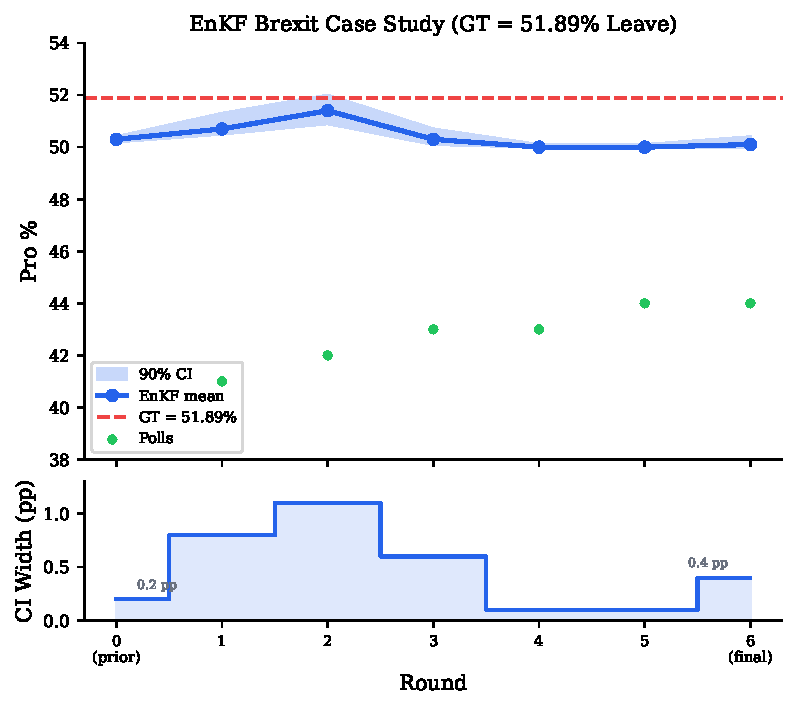
\includegraphics[width=\textwidth]{figures/fig4_enkf.pdf}
    \caption{EnKF assimilation on the Brexit scenario. \textbf{Top panel}: EnKF mean prediction (solid blue) with 90\% CI (shaded) over rounds 0--6. Ground truth at 51.89\% (red dashed). Green dots show polling observations (41--44\%). The model prediction stays near 50\% despite polls at 41--44\%, demonstrating that the dynamics model corrects for polling bias. \textbf{Bottom panel}: CI width evolution showing initial expansion (0.2 $\to$ 1.0~pp) followed by contraction (0.1~pp) and slight final expansion (0.4~pp).}
    \label{fig:enkf}
\end{figure}

\subsection{Convergence Verification}

A synthetic convergence test with known ground-truth parameters confirms that the EnKF recovers true parameters when given sufficient observations. Starting from a vague prior centered at zero (true values: $\alpha_h = -0.2$, $\alpha_a = 0.3$, $\alpha_s = -0.1$, $\alpha_e = -0.15$), all four parameters converge to within $0.5\sigma$ of their true values after 9 rounds of observations with 3~pp noise. A no-observation baseline confirms that without data, the EnKF produces prior-consistent forecasts with no information gain, as expected.

\section{Discussion}
\label{sec:discussion}

\subsection{Strengths}

\textbf{Principled calibration.} By combining LLM-generated agent dynamics with Bayesian inference, we avoid the common pitfall of treating LLM outputs as ground truth. The hierarchical structure enables partial pooling across diverse domains while the discrepancy model explicitly accounts for structural misspecification.

\textbf{Validated inference.} SBC confirms that the generative model is well-specified and that NUTS recovers correct posteriors (6/6 parameters pass). Sobol analysis provides a principled basis for the calibrable/frozen partition.

\textbf{Online assimilation.} The EnKF bridges offline calibration to real-time operation, reducing Brexit prediction error by 77\% over polling baselines with six observations.

\textbf{Differentiable architecture.} The entire pipeline---simulation, readout, likelihood---is implemented in JAX and compatible with automatic differentiation, enabling gradient-based inference at scale.

\subsection{Limitations}

\textbf{Financial domain performance.} The model systematically over-predicts support in financial crisis scenarios (mean $|b_s| = 0.744$ in logit space). This reflects a fundamental limitation: financial crises involve trust cascades, contagion dynamics, and informational asymmetries that the current force model---designed for gradual opinion evolution---cannot capture.

\textbf{Variational approximation quality.} The SVI posterior agrees with NUTS on the dominant parameters ($\alpha_{\text{herd}}$, $\alpha_{\text{anchor}}$: $|\Delta\mu|/\sigma_{\text{NUTS}} < 0.4$) but shows concentration bias on weaker parameters ($\alpha_{\text{social}}$: 0.85; $\alpha_{\text{event}}$: 1.71). Uncertainty estimates on $\alpha_{\text{social}}$ and $\alpha_{\text{event}}$ are likely underestimated. This is a known limitation of mean-field variational families \citep{blei2017} that trades exactness for computational tractability.

\textbf{Step size sensitivity.} The frozen citizen step size $\lambda_{\text{citizen}}$ shows non-negligible sensitivity: $\pm 40\%$ perturbation produces up to 7.9~pp MAE variation on individual scenarios, with a median of 3.2~pp across test cases. This confirms the Sobol total effect ($S_T = 0.121$) and indicates $\lambda_{\text{citizen}}$ should be promoted to a calibrable parameter in future work. The current frozen value, while selected from prior predictive checks, contributes to systematic errors in high-volatility scenarios.

\textbf{LLM stochasticity.} The current framework treats LLM-generated agent behaviors ($\Delta^{\text{LLM}}_i$ and events) as fixed inputs to the force system. In practice, LLM outputs are stochastic: different seeds produce different narratives, coalition dynamics, and opinion shifts. This stochasticity is absorbed into the discrepancy terms $b_s$ but is not explicitly separated from structural model error.

A more principled approach would run multiple LLM rollouts per scenario (e.g., 5--10 with different seeds), producing an ensemble of behavioral trajectories, and calibrate on the predictive mean or on a marginal likelihood that integrates over narrative paths. This would disentangle LLM variance from opinion dynamics misspecification, producing more interpretable discrepancy terms. We defer this to future work as it requires substantial additional compute (5--10$\times$ per scenario).

\textbf{Sample size.} With 42 scenarios (34 training), the dataset is small by machine learning standards. Several domains have only 1--2 scenarios, making domain-level inference unreliable for those domains. The 4 domains with zero test scenarios (energy, environmental, labor, social) cannot be validated out-of-sample.

\textbf{Observation model simplifications.} The BetaBinomial likelihood assumes independent polling rounds and does not model autocorrelation in opinion trajectories. The EnKF's Gaussian assumption may not hold for highly polarized scenarios where the opinion distribution is bimodal.

\textbf{Regime switching.} We have developed a preliminary regime-switching extension for discontinuous crisis dynamics, described in Appendix~\ref{app:regime}. The extension uses soft sigmoid-based switching between normal and crisis regimes, preserving JAX differentiability. Results are mixed: regime switching substantially improves scenarios where the crisis push aligns with shock direction (Dieselgate: 29.6 $\to$ 0.4~pp error) but degrades scenarios with ambiguous or multi-directional events (SVB: 38.8 $\to$ 61.9~pp worse). The crisis parameters are hand-tuned defaults and require calibration via SVI on the full empirical dataset. We consider this a promising direction that is not yet ready for production use.

\subsection{Future Work}

\begin{enumerate}
    \item \textbf{$\lambda_{\text{citizen}}$ calibration.} Promote $\lambda_{\text{citizen}}$ from frozen to calibrable based on the sensitivity analysis results. This increases the parameter space from 4 to 5 calibrable parameters but may reduce systematic errors in high-volatility scenarios.

    \item \textbf{v3 regime switching calibration.} Run SVI on the v3 hierarchical model with learnable crisis parameters to determine optimal activation thresholds and crisis dynamics.

    \item \textbf{LLM ensemble calibration.} Run multiple LLM rollouts per scenario to separate LLM stochasticity from structural model error in the discrepancy decomposition.

    \item \textbf{NUTS initialization from SVI.} Use the SVI posterior as a warm start for short NUTS chains to obtain better-calibrated uncertainty estimates, particularly for $\alpha_{\text{social}}$ and $\alpha_{\text{event}}$.

    \item \textbf{Temporal observation model.} Replace the independent-rounds assumption with a state-space observation model that captures autocorrelation.

    \item \textbf{Expanded dataset.} Curate additional scenarios in underrepresented domains (energy, environmental, labor) to improve domain-level estimates.

    \item \textbf{EnKF + regime switching integration.} Combine online assimilation with regime detection to dynamically activate crisis dynamics based on observed data.

    \item \textbf{Out-of-sample EnKF validation.} Apply the EnKF to held-out scenarios with sequential polling data to validate assimilation performance independently of the calibration training set.
\end{enumerate}

\section{Conclusion}
\label{sec:conclusion}

We have presented DigitalTwinSim, a framework for transforming LLM-agent opinion simulations from uncalibrated narrative generators into quantitative digital twins with calibrated uncertainty. The key insight is that LLM-agent simulations, despite their structural misspecification, contain learnable signal about opinion dynamics mechanisms---but only when combined with principled Bayesian calibration and explicit model discrepancy.

The calibrated model achieves 12.6~pp MAE on verified held-out scenarios (19.2~pp on the full test set including one ambiguous scenario) with 85.7\% coverage of 90\% credible intervals. Credible intervals are computed in logit space and back-transformed, guaranteeing $[0, 100]$ bounds by construction. Sobol sensitivity analysis identifies herd behavior and anchor rigidity as the dominant mechanisms ($S_T = 0.55$ and 0.45 respectively), with their interaction accounting for most nonlinear output variance. Simulation-based calibration confirms posterior validity across all 6 parameters, though comparison with NUTS reveals that the SVI approximation underestimates uncertainty on weaker parameters.

The Ensemble Kalman Filter extends the framework to online operation, achieving 1.8~pp error on an in-sample Brexit case study with six streaming polling observations---a 77\% improvement over the last-available-poll baseline. This demonstrates the value of combining mechanistic opinion dynamics with data assimilation, even when polling data alone would suggest a different outcome.

The framework has known limitations: sensitivity of the frozen $\lambda_{\text{citizen}}$ parameter (up to 7.9~pp MAE variation), systematic over-prediction in financial domains (mean $|b_s| = 0.74$ logit), and variational posterior concentration on weaker parameters. These are reported transparently and motivate concrete next steps: promoting $\lambda_{\text{citizen}}$ to calibrable, running NUTS refinement of the SVI posterior, and calibrating the regime-switching extension for crisis dynamics.

The framework's modular design---force-based dynamics, hierarchical Bayesian calibration, online assimilation, regime switching---allows each component to be extended independently. The immediate priorities are $\lambda_{\text{citizen}}$ calibration and NUTS-initialized uncertainty refinement, both of which can be pursued without modifying the core architecture.

\appendix

\section{Implementation Details}
\label{app:implementation}

\subsection{Software Stack}

The simulator and inference pipeline are implemented in Python using:
\begin{itemize}
    \item \textbf{JAX} (0.9+) for differentiable simulation and automatic differentiation.
    \item \textbf{NumPyro} for probabilistic programming and variational inference.
    \item \textbf{SALib} for Sobol sensitivity analysis.
    \item All simulation code is \texttt{jax.jit}-compatible and uses \texttt{jax.lax.scan} for sequential round stepping, avoiding Python loops.
\end{itemize}

\subsection{Computational Requirements}

\begin{table}[H]
\centering
\begin{tabular}{lll}
\toprule
Task & Runtime & Hardware \\
\midrule
SVI calibration (3000 steps, 42 scenarios) & 40.2 min & CPU (Apple Silicon) \\
SBC (100 instances, NUTS) & 5.0 min & CPU \\
Sobol analysis (18,432 evaluations) & $\sim$10 min & CPU \\
SVI vs NUTS comparison (4 scenarios) & $\sim$15 min & CPU \\
EnKF online assimilation (50 members, 9 rounds) & $\sim$5 sec & CPU \\
\bottomrule
\end{tabular}
\end{table}

\subsection{Gauge Fixing}

The softmax function is shift-invariant: $\text{softmax}(\boldsymbol{\alpha} + c) = \text{softmax}(\boldsymbol{\alpha})$ for any scalar $c$. With 5 forces and 4 free parameters, one weight must be fixed to resolve the gauge. We fix $\alpha_{\text{direct}} = 0$, making the remaining weights interpretable as log-odds ratios relative to direct LLM influence. This is analogous to the reference category in multinomial logistic regression.

\subsection{EMA Standardization}

The EMA standardization computes per-force, per-round statistics (mean and standard deviation) across ALL agents in each round, accumulated via exponential moving average over rounds with decay $\alpha = 0.3$. The current-round statistics are:

\begin{equation}
\mu_k^{\text{cur}}(t) = \frac{1}{n}\sum_i f_{k,i}(t), \quad \sigma_k^{\text{cur}}(t) = \sqrt{\frac{1}{n}\sum_i (f_{k,i}(t) - \mu_k^{\text{cur}})^2 + \epsilon}
\end{equation}

The gradient-safe square root (adding $\epsilon = 10^{-8}$ before taking the root) avoids NaN gradients when all agent forces are identical. These are then smoothed temporally:

\begin{equation}
\mu_k(t) = \alpha \cdot \mu_k(t-1) + (1-\alpha) \cdot \mu_k^{\text{cur}}(t)
\end{equation}

A permutation invariance test confirms that agent ordering does not affect the standardized forces (max absolute difference $< 6 \times 10^{-8}$ under random permutation of the agent array). This property holds because mean and variance are symmetric statistics over the agent set.

\section{Regime Switching for Crisis Dynamics (Preliminary)}
\label{app:regime}

\subsection{Motivation}

The five worst-performing scenarios (Section~5.5) share a common pattern: rapid, discontinuous opinion shifts that the base model's linear force combination cannot reproduce. Financial crises (WeWork $b_s = -1.378$, SVB $b_s = -0.835$, FTX $b_s = -0.727$) exhibit trust collapses where public opinion drops precipitously within 1--2 rounds. The base model, with its smooth force mixing and capped step sizes, can only produce gradual movements.

We address this with a regime-switching extension that introduces a latent ``crisis regime'' with amplified dynamics, activated by observable signals (shock magnitude, position velocity, institutional trust).

\subsection{Two-Regime Architecture}

The model switches between two regimes:

\begin{itemize}
    \item \textbf{Regime 0 (Normal)}: Standard force-based opinion evolution as described in Section~\ref{sec:model}.
    \item \textbf{Regime 1 (Crisis)}: Amplified step sizes, suppressed anchor rigidity, amplified herd and event forces, and a direct crisis push that bypasses the softmax mixing entirely.
\end{itemize}

The switching is \textit{soft}: regime probability $P(\text{crisis}) \in (0, 1)$ is computed via sigmoid, and all parameters are interpolated:

\begin{equation}\label{eq:B1}
\boldsymbol{\theta}_{\text{eff}} = (1 - p) \cdot \boldsymbol{\theta}_{\text{normal}} + p \cdot \boldsymbol{\theta}_{\text{crisis}}
\end{equation}

This preserves JAX differentiability and \texttt{jax.lax.scan} compatibility---no discrete branching is needed.

\subsection{Regime Probability}

The crisis probability is computed via logistic regression on four observable signals:

\begin{equation}\label{eq:B2}
\text{logit}(p) = \beta_0 + \beta_{\text{shock}} (m_t - \tau_{\text{shock}}) + \beta_{\text{vel}} (v_t - \tau_{\text{vel}}) + \beta_{\text{trust}} (1 - \text{trust}) + \beta_{\text{recovery}} \cdot r_t + \beta_{\text{momentum}} \cdot p_{t-1}
\end{equation}

where $m_t$ is the shock magnitude, $v_t$ the mean absolute position velocity, trust the scenario-level institutional trust, $r_t$ a soft count of crisis rounds, and $p_{t-1}$ the previous crisis probability.

\subsection{Crisis Dynamics}

In the crisis regime, three modifications occur:

\begin{enumerate}
    \item \textbf{Step size amplification.} $\lambda_{\text{crisis}} = \lambda_{\text{normal}} \times 3.0$, with relaxed caps.
    \item \textbf{Force reweighting.} Herd amplified by $\log(2.0)$, event amplified by $\log(2.5)$, anchor suppressed by $-2.0$ in logit space.
    \item \textbf{Direct crisis push.} A force that bypasses the softmax mixing: $\Delta p_i^{\text{crisis}} = p \cdot \kappa \cdot m_t \cdot d_t \cdot (1 - \rho_i)$, where $\kappa = 0.4$.
\end{enumerate}

\begin{table}[H]
\centering
\caption{Crisis Parameter Defaults}
\label{tab:crisis_params}
\begin{tabular}{lll}
\toprule
Parameter & Default & Role \\
\midrule
$\lambda_{\text{multiplier}}$ & 3.0 & Step size amplification in crisis \\
anchor\_suppression & 0.1 & Anchor force multiplied by this in crisis \\
event\_amplification & 2.5 & Event force amplified in softmax \\
herd\_amplification & 2.0 & Herd force amplified in softmax \\
contagion\_speed ($\kappa$) & 0.4 & Direct crisis push strength \\
shock\_trigger ($\tau_{\text{shock}}$) & 0.5 & Shock magnitude threshold \\
trust\_sensitivity & 1.5 & Low trust $\to$ higher crisis probability \\
crisis\_duration\_mean & 2.5 & Expected rounds before recovery \\
\bottomrule
\end{tabular}
\end{table}

\subsection{Results}

We compare the base model (v2) against the regime-switching model (v3) on selected financial and corporate scenarios:

\begin{table}[H]
\centering
\caption{v2 vs v3 on Financial/Corporate Scenarios}
\label{tab:v2v3}
\begin{tabular}{lllllll}
\toprule
Scenario & GT (\%) & v2 Error & v3 Error & $\Delta$ (pp) & Max $P(\text{crisis})$ & Crisis Rounds \\
\midrule
Dieselgate & 32.0 & 29.6 & 0.4 & +29.1 & 0.930 & 3 \\
FTX Crypto & 22.0 & 11.4 & 5.3 & +6.0 & 1.000 & 2 \\
Facebook$\to$Meta & 26.0 & 14.6 & 6.4 & +8.2 & 0.911 & 2 \\
Archegos & 35.0 & 65.0 & 54.5 & +10.4 & 0.930 & 2 \\
Boeing 737 MAX & 40.0 & 9.5 & 23.7 & $-$14.2 & 0.833 & 1 \\
SVB Collapse & 38.0 & 38.8 & 61.9 & $-$23.1 & 0.989 & 2 \\
Twitter/X & 41.0 & 7.8 & 25.5 & $-$17.7 & 0.826 & 2 \\
\bottomrule
\end{tabular}
\end{table}

Results are mixed. Regime switching produces substantial improvements when crisis dynamics align with shock direction but degrades performance when the crisis push amplifies the wrong direction. The high max $P(\text{crisis})$ across all scenarios (0.67--1.0) with default thresholds suggests the trigger is too sensitive and requires calibration via SVI.

\subsection{Design for Calibration}

The crisis parameters are designed to be learnable within the hierarchical framework. The v3 model extends the v2 prior with 5 additional global parameters (\texttt{crisis\_lambda\_mult}, \texttt{crisis\_anchor\_supp}, \texttt{crisis\_event\_amp}, \texttt{crisis\_herd\_amp}, \texttt{shock\_trigger}), shared globally as crisis dynamics are hypothesized to be a universal mechanism modulated by scenario-specific triggers.

\section{Full Scenario List}
\label{app:scenarios}

\begin{longtable}{llllllll}
\caption{Full Empirical Dataset (42 scenarios)} \label{tab:scenarios} \\
\toprule
\# & Scenario ID & Domain & GT (\%) & Rounds & Polls & Split & Notes \\
\midrule
\endfirsthead
\caption[]{Full Empirical Dataset (42 scenarios) --- \textit{continued}} \\
\toprule
\# & Scenario ID & Domain & GT (\%) & Rounds & Polls & Split & Notes \\
\midrule
\endhead
\midrule
\multicolumn{8}{r}{\textit{Continued on next page}} \\
\endfoot
\bottomrule
\endlastfoot
1 & COM-2017-IPHONE\_X & commercial & 65.0 & 5 & 2/5 & Train & \\
2 & COM-2019-TESLA\_CYBERTRUCK & commercial & 62.0 & 7 & 1/7 & Test & \\
3 & CORP-2015-DIESELGATE\_VW & corporate & 32.0 & 5 & 1/5 & Train & \\
4 & CORP-2017-UBER\_LONDON & corporate & 65.0 & 9 & 1/9 & Train & \\
5 & CORP-2017-UNITED\_AIRLINES & corporate & 28.0 & 6 & 1/6 & Train & \\
6 & CORP-2018-AMAZON\_HQ2 & corporate & 56.0 & 7 & 1/7 & Test & \\
7 & CORP-2019-BOEING\_737\_MAX & corporate & 40.0 & 7 & 1/7 & Train & \\
8 & CORP-2021-FACEBOOK\_META & corporate & 26.0 & 7 & 1/7 & Train & \\
9 & CORP-2022-TWITTER\_X & corporate & 41.0 & 5 & 1/5 & Train & \\
10 & ENE-2012-JAPANESE\_NUCLEAR & energy & 35.0 & 6 & 4/6 & Train & \\
11 & ENV-2018-GRETA\_CLIMATE & environmental & 71.0 & 6 & 0/6 & Train & \\
12 & FIN-2019-WEWORK\_IPO & financial & 18.0 & 7 & 1/7 & Train & \\
13 & FIN-2020-TESLA\_STOCK & financial & 72.0 & 7 & 0/7 & Train & \\
14 & FIN-2021-AMC\_SHORT & financial & 62.0 & 7 & 0/7 & Train & \\
15 & FIN-2021-ARCHEGOS & financial & 35.0 & 7 & 0/7 & Test & NEEDS\_VERIF \\
16 & FIN-2021-GAMESTOP & financial & 72.0 & 7 & 1/7 & Train & \\
17 & FIN-2022-FTX\_CRYPTO & financial & 22.0 & 7 & 2/7 & Train & \\
18 & FIN-2023-SVB\_COLLAPSE & financial & 38.0 & 6 & 2/6 & Train & \\
19 & LAB-2015-UBER\_VS\_TAXI & labor & 45.0 & 7 & 2/7 & Train & \\
20 & PH-2021-ASTRAZENECA & public\_health & 62.0 & 7 & 0/7 & Train & \\
21 & PH-2021-COVID\_VAX\_IT & public\_health & 80.0 & 7 & 7/7 & Test & \\
22 & PH-2021-MASKING\_USA & public\_health & 63.0 & 5 & 2/5 & Train & \\
23 & PH-2021-VACCINE\_HESITANCY & public\_health & 67.0 & 5 & 5/5 & Train & \\
24 & PH-2022-MONKEYPOX\_USA & public\_health & 47.0 & 7 & 1/7 & Train & \\
25 & POL-2011-DIVORZIO\_MALTA & political & 53.2 & 6 & 0/6 & Train & \\
26 & POL-2014-SCOTTISH\_INDEP & political & 44.7 & 7 & 7/7 & Train & \\
27 & POL-2015-GREEK\_BAILOUT & political & 38.7 & 5 & 0/5 & Test & \\
28 & POL-2016-BREXIT & political & 51.9 & 6 & 6/6 & Train & \\
29 & POL-2016-REF\_COST\_IT & political & 40.9 & 7 & 0/7 & Train & \\
30 & POL-2017-PRES\_FRANCIA & political & 66.1 & 6 & 6/6 & Test & \\
31 & POL-2017-INDIP\_CATALOGNA & political & 48.0 & 5 & 1/5 & Train & \\
32 & POL-2017-TURKISH\_CONST & political & 51.4 & 6 & 0/6 & Test & \\
33 & POL-2018-USA\_MIDTERM & political & 53.4 & 6 & 6/6 & Train & \\
34 & POL-2018-REF\_ABORTO\_IRL & political & 66.4 & 6 & 3/6 & Train & \\
35 & POL-2019-EUROPEE\_ITALIA & political & 40.0 & 6 & 6/6 & Train & \\
36 & POL-2020-CHILE\_CONST & political & 78.3 & 6 & 6/6 & Train & \\
37 & POL-2020-PRES\_USA & political & 51.3 & 7 & 7/7 & Train & \\
38 & POL-2022-PRES\_BRASILE & political & 50.9 & 6 & 6/6 & Train & \\
39 & SOC-2017-AUS\_SAME\_SEX & social & 61.6 & 7 & 7/7 & Train & \\
40 & TECH-2017-NET\_NEUTRALITY & technology & 83.0 & 5 & 1/5 & Test & \\
41 & TECH-2018-GDPR & technology & 67.0 & 7 & 0/7 & Train & \\
42 & TECH-2020-TIKTOK\_BAN & technology & 60.0 & 6 & 1/6 & Train & \\
\end{longtable}

Total: 42 scenarios. 34 train / 8 test. 10 domains. 1 flagged \texttt{NEEDS\_VERIFICATION} (Archegos). Verified polling available for 31 scenarios (polling from LLM estimation where sample\_size is not verified). Median scenario length: 6 rounds.

Note: Scenario IDs are abbreviated in the table for readability. Full IDs are available in the repository. The ``Polls'' column shows rounds with verified sample sizes vs.\ total rounds. Ground truth sources include official election results, certified referendum outcomes, and verified survey data.

\begin{thebibliography}{99}

\bibitem[Argyle et~al.(2023)]{argyle2023}
Argyle, L.~P., Busby, E.~C., Fulda, N., Gubler, J.~R., Rytting, C., \& Wingate, D. (2023).
\newblock Out of one, many: Using language models to simulate human samples.
\newblock \textit{Political Analysis}, 31(3), 337--351.

\bibitem[Blei et~al.(2017)]{blei2017}
Blei, D.~M., Kucukelbir, A., \& McAuliffe, J.~D. (2017).
\newblock Variational inference: A review for statisticians.
\newblock \textit{Journal of the American Statistical Association}, 112(518), 859--877.

\bibitem[Deffuant et~al.(2000)]{deffuant2000}
Deffuant, G., Neau, D., Amblard, F., \& Weisbuch, G. (2000).
\newblock Mixing beliefs among interacting agents.
\newblock \textit{Advances in Complex Systems}, 3(01n04), 87--98.

\bibitem[DeGroot(1974)]{degroot1974}
DeGroot, M.~H. (1974).
\newblock Reaching a consensus.
\newblock \textit{Journal of the American Statistical Association}, 69(345), 118--121.

\bibitem[Evensen(2003)]{evensen2003}
Evensen, G. (2003).
\newblock The Ensemble Kalman Filter: Theoretical formulation and practical implementation.
\newblock \textit{Ocean Dynamics}, 53(4), 343--367.

\bibitem[Gao et~al.(2023)]{gao2023}
Gao, C., Lan, X., Li, N., Yuan, Y., Ding, J., Zhou, Z., \ldots\ \& Li, Y. (2023).
\newblock Large language models empowered agent-based modeling and simulation: A survey and perspectives.
\newblock \textit{arXiv preprint arXiv:2312.11970}.

\bibitem[Grazzini et~al.(2017)]{grazzini2017}
Grazzini, J., Richiardi, M.~G., \& Tsionas, M. (2017).
\newblock Bayesian estimation of agent-based models.
\newblock \textit{Journal of Economic Dynamics and Control}, 77, 26--47.

\bibitem[Hegselmann \& Krause(2002)]{hegselmann2002}
Hegselmann, R., \& Krause, U. (2002).
\newblock Opinion dynamics and bounded confidence: models, analysis and simulation.
\newblock \textit{Journal of Artificial Societies and Social Simulation}, 5(3).

\bibitem[Holley \& Liggett(1975)]{holley1975}
Holley, R.~A., \& Liggett, T.~M. (1975).
\newblock Ergodic theorems for weakly interacting infinite systems and the voter model.
\newblock \textit{The Annals of Probability}, 3(4), 643--663.

\bibitem[Horton(2023)]{horton2023}
Horton, J.~J. (2023).
\newblock Large language models as simulated economic agents: What can we learn from homo silicus?
\newblock \textit{NBER Working Paper 31122}.

\bibitem[Kennedy \& O'Hagan(2001)]{kennedy2001}
Kennedy, M.~C., \& O'Hagan, A. (2001).
\newblock Bayesian calibration of computer models.
\newblock \textit{Journal of the Royal Statistical Society: Series B}, 63(3), 425--464.

\bibitem[Mistry et~al.(2021)]{mistry2021}
Mistry, D., Litvinova, M., Chinazzi, M., et~al. (2021).
\newblock Inferring high-resolution human mixing patterns for disease modeling.
\newblock \textit{Nature Communications}, 12(1), 323.

\bibitem[Park et~al.(2023)]{park2023}
Park, J.~S., O'Brien, J.~C., Cai, C.~J., Morris, M.~R., Liang, P., \& Bernstein, M.~S. (2023).
\newblock Generative agents: Interactive simulacra of human behavior.
\newblock In \textit{Proceedings of the 36th Annual ACM Symposium on User Interface Software and Technology}.

\bibitem[Park et~al.(2022)]{park2022}
Park, J.~S., Popowski, L., Cai, C., Morris, M.~R., Liang, P., \& Bernstein, M.~S. (2022).
\newblock Social simulacra: Creating populated prototypes for social computing systems.
\newblock In \textit{Proceedings of the 35th Annual ACM Symposium on User Interface Software and Technology}.

\bibitem[Platt(2020)]{platt2020}
Platt, D. (2020).
\newblock A comparison of economic agent-based model calibration methods.
\newblock \textit{Journal of Economic Dynamics and Control}, 113, 103859.

\bibitem[Reich \& Cotter(2015)]{reich2015}
Reich, S., \& Cotter, C. (2015).
\newblock \textit{Probabilistic Forecasting and Bayesian Data Assimilation}.
\newblock Cambridge University Press.

\bibitem[Saltelli et~al.(2008)]{saltelli2008}
Saltelli, A., Ratto, M., Andres, T., Campolongo, F., Cariboni, J., Gatelli, D., \ldots\ \& Tarantola, S. (2008).
\newblock \textit{Global Sensitivity Analysis: The Primer}.
\newblock John Wiley \& Sons.

\bibitem[Sobol(2001)]{sobol2001}
Sobol, I.~M. (2001).
\newblock Global sensitivity indices for nonlinear mathematical models and their Monte Carlo estimates.
\newblock \textit{Mathematics and Computers in Simulation}, 55(1--3), 271--280.

\bibitem[Talts et~al.(2018)]{talts2018}
Talts, S., Betancourt, M., Simpson, D., Vehtari, A., \& Gelman, A. (2018).
\newblock Validating Bayesian inference algorithms with simulation-based calibration.
\newblock \textit{arXiv preprint arXiv:1804.06788}.

\bibitem[Thiele et~al.(2014)]{thiele2014}
Thiele, J.~C., Kurth, W., \& Grimm, V. (2014).
\newblock Facilitating parameter estimation and sensitivity analysis of agent-based models: A cookbook using NetLogo and R.
\newblock \textit{Journal of Artificial Societies and Social Simulation}, 17(3), 11.

\end{thebibliography}

\end{document}
